\chapter{Выпуклые структуры}

\section{Выпуклые множества}

\subsection{Выпуклые множества и теоремы отделимости}


    Выпуклые множества, а также выпуклые и вогнутые функции,
    играют важнейшую роль в теории экстремальных задач
    и многих важнейших разделах
    математической экономики. Глубокое знакомство с теорией выпуклых
    множеств является необходимым для всякого, кто желает стать
    специалистом в области экономической теории.

    Дадим основные определения.

    \emph{Отрезком}, соединяющим две точки $\vc{x}'$ и $\vc{x}''$ из
    пространства $\R^{n}$, называется множество
    \[\{\vc{x}\in\R^{n} \ | \ \vc{x}=(1-\theta)\vc{x}'+\theta\vc{x}'', \ \theta\in[0,1]\}\]
    всех векторов вида
    $(1-\theta)\vc{x}'+\theta\vc{x}''$
    при $\theta$, пробегающем все
    значения от $0$ до $1$ (включая $0$ и $1$).
    Если некоторая точка $\vc{x}\in\R^{n}$ представима в виде
    $\vc{x}=(1-\theta)\vc{x}'+\theta\vc{x}''$ при некотором фиксированном
    $\theta\in[0,1]$, то эта точка называется \emph{выпуклой комбинацией} $\vc{x}'$ и
    $\vc{x}''$ (с весами $1-\theta$ и $\theta$). Тем самым отрезок, соединяющий $\vc{x}'$ и
    $\vc{x}''$ представляет собой множество всех выпуклых комбинаций
    $\vc{x}'$ и $\vc{x}''$.

    Выпуклая комбинация векторов $\vc{x}'$ и $\vc{x}''$ с весами
    $1-\theta=0$ и $\theta=1$ --- это, очевидно, вектор $\vc{x}''$,
    который можно для иллюстративности представить как
    \[\vc{x}'+\theta(\vc{x}''-\vc{x}'), \ \theta=1,\]
    (см. Рис.??????), а выпуклая комбинация $\vc{x}'$ и
    $\vc{x}''$ с весами
    $1-\theta=1/2$ и $\theta=1/2$ --- это вектор
\[
    \frac{\vc{x}'+\vc{x}''}{2}=\vc{x}'+\frac{1}{2}(\vc{x}''-\vc{x}'),
\]
    лежащий ровно посередине отрезка, соединяющего точки $\vc{x}'$ и $\vc{x}''$.
    (см. Рис. ?????).


    Множество $\st{X}\subset\R^{n}$ называется \emph{выпуклым}, если с
    любыми своими двумя точками $\vc{x}'$ и $\vc{x}''\!$ оно
    содержит весь отрезок, соединяющий эти две точки.













\input{pics/segment.TpX}












Примеры выпуклого и невыпуклого множества приведены на Рис.~
\ref{fig:nonconvex}.

\begin{figure} \centering
\includegraphics[width=13cm,height=5cm]{convex}
\caption{Выпуклые и невыпуклые множества \cite{Gale:1963}}
\label{fig:nonconvex}
\end{figure}

\begin{exer}
Убедитесь в том, что пересечение  любого (конечного или
бесконечного) числа выпуклых множеств также является выпуклым
множеством, а объединение может и не быть выпуклым множеством.
\end{exer}

\begin{exer}
    Пусть $a(\vc{x})$ --- линейный функционал, заданный на $\R^{n}$.
    Проверьте, что при заданном  $\gamma\in\R$
    выпуклы следующие множества:
    \[\{\vc{x}\in\R^{n} \ | \ a(\vc{x})=\gamma\},\]
    \[\{\vc{x}\in\R^{n} \ | \ a(\vc{x})>\gamma\},\]
    \[\{\vc{x}\in\R^{n} \ | \ a(\vc{x})\leq\gamma\}.\]
\end{exer}



    Пусть нам заданы ненулевой линейны функционал $p(\vc{x})$, заданный на $\R^{n}$,
    и число $\gamma $.
    Множество $\st{H}$, определяемое как
\[
\st{H}_{p,\gamma}= \{ \vc{x}\in \R^n: p(\vc{x}) = \gamma\}
\]
    называется гиперплоскостью в $\R^n$, а множества
\[
\st{H}_{p,\gamma}^{-}= \{ \vc{x}\in \R^n: p(\vc{x})\leq\gamma\}
\]
    и
\[
\st{H}_{p,\gamma}^{+}= \{ \vc{x}\in \R^n: p(\vc{x})\geq\gamma\}
\]
    --- (замкнутыми) полупространствами, ею порождаемыми.


    Примерами гиперплоскостей в двумерном и трехмерном пространства
    являются соответственно \emph{прямая} и \emph{плоскость} (см. Рис.
    ~\ref{fig:Hplanes_exam} ВТОРОЙ РИСУНОК НЕХОРОШ!!!!). Очевидно, что вектор $\vc{p}$, задающий
    линейный функционал $p(\vc{x})$, перпендикулярен соответствующей прямой или плоскости и
    направлены в сторону возрастания функции $p(\vc{x})$.

\begin{figure}
\centering
\renewcommand{\thesubfigure}{\asbuk{subfigure})}
\subfigure[Прямая]{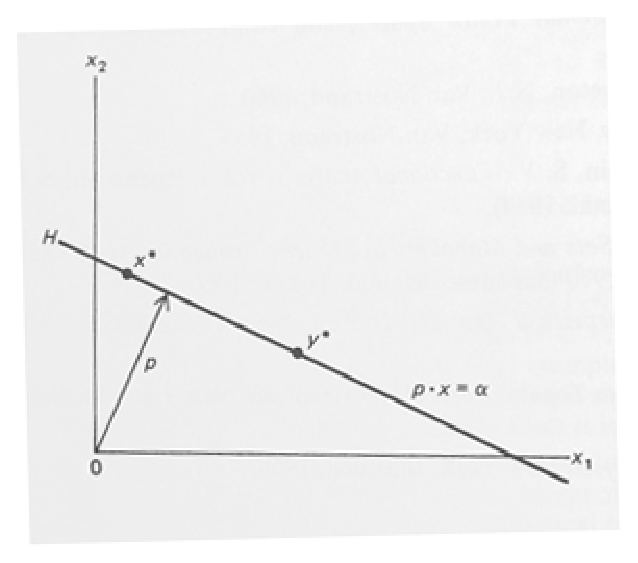
\includegraphics[width=0.47\textwidth]{line}}\hfill
\subfigure[Плоскость]{\includegraphics[width=0.47\textwidth]{3dplane}}
\caption{Примеры гиперплоскостей}\label{fig:Hplanes_exam}
\end{figure}



Изменяя значение $\gamma$ (сдвигая гиперплоскость), мы получаем
целое семейство гиперплоскостей (см. Рис.~\ref{fig:hypermap}).

\input{pics/hypermap.TpX}


    Важнейшая роль выпуклых множество в математической экономике и теории экстремальных задач
    обусловлена тем, что для них справедливы так называемые теоремы отделимости.
    Есть несколько различных формулировок теорем отделимости. Мы приведем здесь только те из них,
    которые понадобятся нам в дальнейшем. Их доказательства мы приводить не будем в надежде на то,
    что геометрически они выглядят довольно правдоподобными.

    Два множества $\st{X}$ и $\st{Y}$ из $\R^n$ называются
    \emph{отделимыми}, если существует такая гиперплоскость
    $\st{H}_{p,\gamma}$, называемая \emph{разделяющей}, что множество
    $\st{X}$ лежит в одном
    из замкнутых полупространств, порожденных этой гиперплоскостью,
    а множество $\st{Y}$ --- во втором. Иными словами, множества $\st{X}$ и
    $\st{Y}$ отделимы, если существуют такой ненулевой линейный функционал $p(\vc{x})$,
    и число $\gamma$, что
\[
    p(\vc{x})\leq\gamma\leq p(\vc{y}) \ \forall \vc{x}\in\st{X} \ \forall \vc{y}\in\st{Y}.
\]




\begin{teo}[отделимости]
  \label{teo-otd-1}
    Предположим, что $\st{X}$ и $\st{Y}$ --- выпуклые множества из
    $\R^n$, причем хотя бы одно из них, скажем, $\st{Y}$, имеет
    непустую внутренность (\remrk{что такое внутренность????}) $\emph{int}\st{Y}$. Если
    $\st{X}\cap\emph{int}\st{Y}=\emptyset$, то множества $\st{X}$ и
    $\st{Y}$ отделимы.
\end{teo}

     Подчеркнем, что в
    сформулированной теореме не требуется, чтобы множества не пересекались. Важно, чтобы
    одно из двух множеств не пересекалось с внутренностью другого, если, конечно, эта
    внутренность сама не являлась пустым множеством (см. \remrk{РИС}).
    Безусловно, предположение о том, что оба множества, $\st{X}$ и $\st{Y}$,
    являются выпуклыми, является крайне существенным, что проиллюстрировано \remrk{РИС}.


    Пусть $\st{X}$ --- некоторое множество из $\R^{n}$ и точка
    $\vc{\hat{x}}$ принадлежит границе этого множества. Гиперплоскость
    $\st{H}_{p,\gamma}$ называется \emph{опорной} к множеству $\st{X}$
    в точке $\vc{\hat{x}}$, если эта точка принадлежит
    данной гиперплоскости, а само множество $\st{X}$ содержится в
    полупространстве $\st{H}_{p,\gamma}^{-}$, т.е. если
    \[\gamma=p(\vc{\hat{x}})\geq p(\vc{x}) \ \forall x\in\st{X}.\]

    Заметим, что последнее неравенство говорит, в частности, что
    если точка $\vc{\hat{x}}$  принадлежит множеству $\st{X}$
    (а это действительно так, если это множество замкнуто),
    то она  представляет собой решение задачи
\begin{equation}
    \label{max-lin-na-vip}
    p(\vc{x})\rightarrow\max, \ \vc{x}\in\st{X},
\end{equation}
    причем значением этой задачи является число $\gamma$. Подчеркнем также,
    что, формально говоря, опорная к множеству $\st{X}$
    в точке $\vc{\hat{x}}$ гиперплоскость представляет собой
    гиперплоскость, разделяющую множество $\st{X}$ и множество,
    состоящее из единственной точки $\vc{\hat{x}}$ (\remrk{РИС}).

\begin{teo}[об опорной гиперплоскости]
    \label{teo-op-gip}
    Если $\st{X}$ --- выпуклое множество, то для любой его граничной (\remrk{????})
    точки $\vc{\hat{x}}$  найдется гиперплоскость, опорная в этой точке
    к данному множеству.
\end{teo}

    Из теоремы об опорной гиперплоскости следует, что любая
    граничная точка выпуклого замкнутого множества $\st{X}$ представляет
    собой решение некоторой задачи вида (\ref{max-lin-na-vip}). В то
    же время, очевидно, что любое решение такой задачи является
    граничной точкой $\st{X}$. Заметим, что в случае, когда
    множество $\st{X}$ имеет непустую внутренность, теорема об
    опорной гиперплоскости вытекает из теоремы отделимости.

    Далее нам понадобится еще одна теорема, которая говорит, что
    если точка $\vc{\hat{x}}$ не принадлежит выпуклому замкнутому
    множеству $\st{X}$, то $\vc{\hat{x}}$ <<строго>> отделима от
    $\st{X}$ с помощью некоторой гиперплоскости $\st{H}_{p,\gamma}$ (\remrk{РИС ?????}).


\begin{teo}\label{strog-otdotochki}
    Пусть $\st{X}$ --- выпуклое замкнутое множество, а точка
    $\vc{\hat{x}}$  не принадлежит $\st{X}$. Тогда существует такой
    ненулевой линейный функционал $p(\vc{x})$ и число
     $\gamma$, такие что
    \[p(\vc{x})<p(\vc{\hat{x}}) \ \forall \vc{x}\in\st{X}.\]
\end{teo}

\begin{exer}
    Докажите, что любое замкнутое выпуклое множество $\st{X}$ представляет
    собой пересечение всех полупространств
    $\st{H}_{p,\gamma}^{-}$, порождаемых опорными к $\st{X}$
    гиперплоскостями.


\end{exer}


\section{Лемма Фаркаша}

    В качестве приложения одной из только что сформулированных теорем, докажем важную
    лемму Фаркаша, которую мы уже использовали в предыдущей главе для доказательства
    некоторых теорем линейного программирования.


    Множество $\st{X}\subset\R^{n}$ называется \emph{\textbf{конусом}}, если для
    любого вектора $\vc{x}\in\st{X}$ и любого числа
    $\lambda\geqslant0$ справедливо включение
     $\lambda\vc{x}\in\st{X}$, т.е. если вместе с любой своей точкой множество
     $\st{X}$ вместе с любой своей точкой содержит проходящий через
     нее луч с началом в нуле (см. рис. ?????, а)
     Если конус $\st{X}$ является выпуклым
     множеством, то он называется \emph{\textbf{выпуклым конусом}} (см. рис. ?????, b).
     Простейшим примером выпуклого конуса является множество $\R_{+}^{n}$.


\begin{exer}
    Докажите, что
    \begin{itemize}
      \item множество $\st{X}$ является выпуклым конусом
    тогда и только тогда, когда для любых векторов $\vc{x'}\in\st{X}$
    и $\vc{x''}\in\st{X}$ и любых чисел $\lambda'\geqslant0$ и
    $\lambda''\geqslant0$ справедливо включение
    $\lambda'\vc{x'}+\lambda''\vc{x''}\in\st{X}$;
      \item пересечение любого числа выпуклых конусов является выпуклым
      конусом;
      \item объединение любого числа выпуклых конусов является конусом,
      но необязательно выпуклым.
    \end{itemize}

\end{exer}


    Пусть $\vc{a^{1}},\ldots,\vc{a^{m}}$ --- конечный набор векторов из
    $\R^{n}$. Вектор вида
    \[\lambda_{1}\vc{a^{1}}+\ldots+\lambda_{m}\vc{a^{m}}\] называется
    \textbf{\emph{линейной комбинацией}} этих векторов. Эта
    линейная комбинация называется \emph{\textbf{неотрицательной}}, если
    $\lambda_{1}\geqslant0,\ldots,\lambda_{m}\geqslant0$ и \emph{\textbf{выпуклой}},
    если $\lambda_{1}\geqslant0,\ldots,\lambda_{m}\geqslant0$ и
    $\lambda_{1}+\ldots+\lambda_{m}=1$. Напомним, что понятие выпуклой комбинации двух точек
    мы уже использовали.




\begin{exer}\label{vipukl-konus}
    Докажите, что
\begin{itemize}
      \item
      множество всевозможных неотрицательных линейных комбинаций конечного набора
      векторов является выпуклым конусом;
      \item
      множество всевозможных выпуклых комбинаций конечного набора
      векторов является выпуклым множеством;
 \end{itemize}
\end{exer}

    Множество всевозможных линейных неотрицательных комбинаций
    конечного набора векторов $\vc{a^{1}},\ldots,\vc{a^{m}}$
    называется конусом, \emph{\textbf{натянутым}} на эти вектора.


    Для доказательства леммы Фаркаша нам понадобится следующая
    техническая лемма. Доказательство этой леммы является несложным, но
    довольно длинным. Поэтому мы его опускаем в надежде на то, что
    сама ее формулировка представляется читателю вполне
    естественной.

\begin{lem}\label{zamkn-konus}
    Конус, натянутый на любой конечный набор векторов, является
    замкнутым множеством.
\end{lem}


    Перейдем к формулировке и доказательству леммы Фаркаша.


\begin{teop}(лемма Фаркаша) \label{lemma-F1}
    Предположим, что нам задан конечный набор векторов
    \[\vc{a_{1}},\ldots,\vc{a_{m}},\]
    лежащих в конечномерном пространстве ${\R}^{n}$. Для любого
    вектора $\vc{d}$ из ${\R}^{n}$ справедлива одна и только одна из двух
    следующих альтернатив:
\begin{itemize}
    \item [1)\ ] либо найдутся числа
    $v_{1}\geq0,\ldots,v_{m}\geq0$, такие что
    \[\vc{d}=v_{1}\vc{a_{1}}+\ldots+v_{m}\vc{a_{m}};\]

    \item [2)\ ] либо существует такой линейный функционал $h(\cdot)$,
    заданный на ${\R}^{n}$, что одновременно выполняются следующие неравенства:
    \[h(\vc{a_{1}})\leq0,\ldots,h(\vc{a_{m}})\leq0,\]
    \[h(\vc{d})>0.\]
\end{itemize}
\end{teop}

    \emph{\textbf{Доказательство.}}
    Рассмотрим конус $\mathbb{K}$, натянутый на вектора
    $\vc{a_{1}},\ldots,\vc{a_{m}}$. Этот конус является выпуклым
    (см. упражнение \ref{vipukl-konus}) и, по
    лемме \ref{zamkn-konus}, замкнутым.

    Возможно одно и только одно из двух следующих соотношений: либо $\vc{d}\in\mathbb{K}$,
    либо $\vc{d}\notin\mathbb{K}$. Включение  $\vc{d}\in\mathbb{K}$
    эквивалентно существованию (\remrk{РИС ?????}) таких неотрицательных чисел
    $v_{1}\geq0,\ldots,v_{m}\geq0$, что
    \[\vc{d}=v_{1}\vc{a_{1}}+\ldots+v_{m}\vc{a_{m}}.\]

    Что касается соотношения $\vc{d}\notin\mathbb{K}$, то с учетом
    теоремы \ref{strog-otdotochki}, оно эквивалентно существованию
    такого линейного функционала $h(\vc{x})$ (\remrk{РИС ?????}), заданного на пространстве $\R^{n}$,
    для которого выполняется следующее соотношение:
\[
    h(\vc{x})< h(\vc{d}) \ \forall \vc{x}\in\mathbb{K}.
\]
    Поскольку $\vc{0}\in\mathbb{K}$, мы имеем: $h(\vc{d})>0$.

    Покажем, что
\[
    h(\vc{x})\leqslant0 \ \forall \vc{x}\in\mathbb{K}.
\]
    Действительно, предположим, что $h(\vc{\bar{x}})>0$ для некоторого
    $\vc{\bar{x}}\in\mathbb{K}$. В этом случае при достаточно
    большом $\lambda>0$ одновременно выполняется неравенство
    $h(\lambda\vc{\bar{x}})>h(\vc{d})$ и включение
    $\lambda\vc{\bar{x}}\in\mathbb{K}$, чего быть не может.

    Нам осталось заметить, что $\vc{a_{j}}\in\mathbb{K}, \ j=1,\ldots,m$ и, значит,
    $h(\vc{a_{j}})\leqslant0, \ j=1,\ldots,m$.
    $\Box$

    Важным следствием доказанной теоремы является следующая лемма.

\begin{lem}\label{lemma-F2}
    Предположим, что нам заданы $r\times s$ матрица $\vc{A}$ и
    $r$-мерный вектор-столбец $\vc{d}$. Справедлива ровно одна из двух
    следующих альтернатив:
\begin{itemize}
    \item [1)\ ] либо найдется $s$-мерный вектор-столбец $\vc{v}\geqq\vc{0}$,
    такой что
    \[\vc{d}=\vc{A}\vc{v};\]

    \item [2)\ ] либо существует такая вектор-строка $\vc{h}$, что
    одновременно выполняются следующие неравенства:
    \[\vc{h}\vc{A}\leqq0, \ \vc{h}\vc{d}>0.\]
    \end{itemize}
\end{lem}
    \textbf{\emph{Доказательство.}}
    Рассмотрим набор $r$-мерных
    вектор-столбцов $\vc{a_{1}},\ldots,\vc{a_{s}}$,  из которых состоит матрица
    $\vc{A}$, и $r$-мерный вектор-столбец $\vc{d}$. По теореме
    \ref{lemma-F1} выполняется ровно одна из двух следующих
    альтернатив:

    --- либо существует такой неотрицательный $s$-мерный
    вектор-столбец
    $\vc{v}=\left(
              \begin{array}{c}
                v_{1} \\
                \vdots \\
                v_{s} \\
              \end{array}
            \right)$,
            что
       \[\vc{d}=v_{1}\vc{a_{1}}+\ldots+v_{s}\vc{a_{s}}=\vc{A}\vc{v},\]
    --- либо найдется такой линейный функционал $h(\vc{x})$,
    заданный на ${\R}^{r}$, что одновременно выполняются следующие неравенства:
    \[h(\vc{d})>0,\]
  \[h(\vc{a_{1}})\leq0,\ldots,h(\vc{a_{m}})\leq0.\]
    Рассмотрим вторую альтернативу.
    Как мы помним, всякий линейный функционал, заданный на пространстве
    $\R^{r}$, состоящем из вектор-столбцов, однозначным образом
    задается некоторой $r$-мерной вектор-строкой. Применительно к
    линейному функционалу $h(\vc{x})$ это значит, что существует
    такая вектор-строка $\vc{h}=(h_{1},\ldots,h_{r})$, что для любого
    вектора $\vc{x}\in\R^{r}$ выполняется равенство
    $\vc{h}\vc{x}=h(\vc{x})$. Для этой вектор-строки мы имеем:
\[
    \vc{h}\vc{d}>0,
\]
\[
    \vc{h}\vc{a_{1}}\leq0,\ldots,\vc{h}\vc{a_{s}}\leq0,
\]
    причем последний набор неравенств мы компактно можем переписать
    в следующем виде:
\[
    \vc{h}\vc{A}\leqq0. \Box
\]

\begin{exer}
    Докажите следующую лемму.
\end{exer}


\begin{lem}\label{lemma-F3}
    Предположим, что нам заданы $s\times r$ матрица $\vc{A}$ и
    $r$-мерный вектор-столбец $\vc{d}$. Справедлива ровно одна из двух
    следующих альтернатив:
\begin{itemize}
    \item [1)\ ] либо найдется $s$-мерный вектор-строка $\vc{v}\geqq\vc{0}$,
    такая что
    \[\vc{d}=\vc{v}\vc{A};\]

    \item [2)\ ] либо существует такой вектор-столбец $\vc{h}$, что
    одновременно выполняются следующие неравенства:
    \[\vc{A}\vc{h}\leqq0, \ \vc{d}\vc{h}>0.\]
    \end{itemize}
\end{lem}

    Заметим, что в научной и учебной литературе иногда под леммой Фаркаша понимают не теорему
    \ref{lemma-F1}, а лемму \ref{lemma-F2} или лемму \ref{lemma-F3}










\newpage

\section{Эффективные точки}

Важную роль в экономическом анализе играет понятие эффективности,
которое несколько отличается от обыденного представления об
эффективности.


УТОЧНИТЬ ОПРЕДЕЛЕНИЯ!!!!!

\begin{dfn}

    Точка ${\vc{\hat x}} \in \st{X} \subset \R^n$ называется

\begin{enumerate}
  \item \textbf{эффективной} точкой множества $\st{X}$, если не существует другой точки $\vc{x} \in
\st{X}$, такой, что $\vc{x} \geq \vc{\hat x}$;

  \item \textbf{слабо эффективной} точкой
множества $\st{X}$, если не существует другой точки $\vc{x} \in
\st{X}$, такой, что $\vc{x} \gg \vc{\hat x}$.

\end{enumerate}
\end{dfn}

    Чтобы пояснить введенные определения, напомним, какой смысл
    имеют неравенства $\geq$ и $\gg$ применительно к векторам. Для
    векторов $\vc{x}=(x_{1},...,x_{n})$ и $\vc{y}=(y_{1},...,y_{n})$
    из пространства $\R^{n}$ неравенство $\vc{x}\gg\vc{y}$
    означает, что
\[
    x_{i}>y_{i}, \ i=1,...,n,
\]
    неравенство $\vc{x}\geqq\vc{y}$ говорит о том, что
\[
    x_{i}\geqslant y_{i}, \ i=1,...,n,
\]
    а соотношение $\vc{x}\geq\vc{y}$ --- о том, что выполняются последние неравенства и $x_{i}>y_{i}$
    хотя бы для одного $i$.
    Мы видим, что точка
    ${\vc{\hat x}} \in \st{X}$ является слабо эффективной, если \emph{не
    найдется} другой точки $\vc{x}$ из множества $\st{X}$,
    превосходящей ${\vc{\hat x}}$ по всем координатам. Точка
    ${\vc{\hat x}} \in \st{X}$ является эффективной, если не найдется другой
    точки $\vc{x}\in\st{X}$, которая не меньше ${\vc{\hat x}}$ по
    всем координатам, причем хотя бы по одной --- строго больше.






Из приведенного выше определения нетрудно видеть, что любая эффективная точка является и
слабо эффективной. Если точка не является слабо эффективной, то она не может быть и
эффективной. В то же время, из того факта, что точка ${\vc{\hat x}}$ является слабо
эффективной, не следует, что она эффективна. (\remrk{РИС?????})





\begin{prop}\label{vzvesh-summa}

Пусть $\st{X} \subset \R^n$ и пусть вектор $\vc{\hat x}$ представляет собой решение задачи

\begin{equation}\label{eq:eff_conditions}
\left\{ \begin{array}{l}
 \vc{p}\vc{x} = p_1x_1 + \ldots + p_n x_n\to \max  \\
 \vc{x} \in \st{X}, \\
 \end{array} \right.
\end{equation}



\begin{enumerate}
\renewcommand{\theenumi}{(\roman{enumi})}
  \item Если $\vc{p} \geq \vc{0}$, то точка $\vc{\hat x} \in \st{X}$ является
  слабо эффективной.
  \item Если $\vc{p} \gg \vc{0}$, то точка $\vc{\hat x} \in \st{X}$ является
  эффективной.
\end{enumerate}

\end{prop}

\begin{proof}

(i) Предположим, что утверждение данного пункта не выполняется. В
этом случае существует $\vc{\bar x} \in \st{X}$ такой, что $\vc{\bar
x} \gg \vc{\hat x}$. Тогда, поскольку $\vc{p} \geq \vc{0}$, получаем
$\vc{p}\vc{\bar x} > \vc{p}\vc{\hat x}$. Однако это противоречит
тому факту, что $\vc{\hat x}$ есть решение задачи
(\ref{eq:eff_conditions}).

(ii) Докажите самостоятельно в качестве \textbf{упражнения}.

\end{proof}



Отметим, что в приведенном предложении не накладывается никаких требований к устройству
множества $\st{X}$. В некотором смысле обратное утверждение требует выпуклости множества
$\st{X}$.



\begin{prop}\label{usl-eff}

Пусть $\st{X} \subset \R^n$ --- выпуклое множество. Если точка ${\vc{\hat x} \in \st{X}}$
является слабо эффективной точкой множества $\st{X}$, то существует вектор ${\vc{p} \geq
\vc{0}}$ из $\R^n$, такой что
\[\vc{p}\vc{\hat x}\geq\vc{p}\vc{x} \ \forall \vc{x}\in\st{X},\]
т.е. $\vc{\hat x}$ есть решение задачи (\ref{eq:eff_conditions}).
\end{prop}

\begin{proof}
Положим
\[
    \st{Y}=\{\vc{y} \in \R^n: \vc{y} \geqq \vc{\hat x}\}.
\]
Множество $\st{Y}$ является выпуклым, причем, как легко проверить,
\[
    \text{int}\st{Y}=\{\vc{y} \in \R^n: \vc{y} \gg \vc{\hat x}\}.
\]

 Поскольку $\vc{\hat x}$
является слабо эффективной точкой множества $\st{X}$, то, как легко заметить,
 $\st{X}\cap\text{int}\st{Y}=\emptyset$. Таким образом, мы имеем два непересекающихся
 выпуклых множества, $\st{X}$ и $\st{Y}$, причем таких, что первое из них не пересекается
 с непустой внутренностью второго (\remrk{РИС?????}).

Значит, по теореме отделимости (теореме \ref{teo-otd-1}) найдутся
ненулевой вектор $\vc{p}=(p_{1},...,p_{n})\in \R^n$ и число
    $\gamma\in \R$ такие, что для любого $\vc{x} \in \st{X}$ и любого $\vc{y}
\in \st{Y}$ выполняются следующие соотношения:

\[
\vc{p} \cdot \vc{x} \leq \gamma \leq \vc{p} \cdot \vc{y}.
\]

    Проверим, что $\vc{p} \geq \vc{0}$. Для этого предположим, что
 это не так и, тем самым, $p_i <0$ для некоторого $i$. Обозначим
 через $\vc{e_{i}}$ вектор из $\R^{n}$, все координаты
 которого, за исключением $i$-й, равны $0$, а $i$-я координата равна
 $1$. Очевидно, $\vc{p}\vc{e_{i}}=p_{i}<0$
    и, следовательно, $\vc{p}(\vc{\hat x}+\vc{e_{i}})<\vc{p}\vc{\hat x}$.
    А этого быть не может, поскольку вектор $\vc{\hat x}+\vc{e_{i}}$ содержится в $\st{Y}$.

    Нам осталось заметить, что, поскольку $\vc{\hat x}$ содержится как в $\st{X}$, так и в
    $\st{Y}$, мы имеем
    $\vc{p} \cdot \vc{\hat x}=\gamma$.
    А это означает, что
    $\vc{\hat x}$ есть решение задачи (\ref{eq:eff_conditions}).
\end{proof}

    Из двух сформулированных предложений вытекает следующая теорема.

\begin{teop}\label{neob-dosti-usl-eff}
    Пусть $\st{X} \subset \R^n$ --- выпуклое замкнутое множество.
    Вектор ${\vc{\hat x} \in \st{X}}$ является слабо эффективной точкой
    множества $\st{X}$ тогда и только тогда, когда то существует вектор
    ${\vc{p} \geq \vc{0}}$, $\vc{p} \in \R^n$, такой что
    \[\vc{p}\vc{\hat x}\geq\vc{p}\vc{x} \ \forall \vc{x}\in\st{X},\]
    т.е. $\vc{\hat x}$ есть решение задачи (\ref{eq:eff_conditions}).
\end{teop}



  Напомнив, что всякая эффективная точка
  является и слабо эффективной, отметим, что нельзя сформулировать аналогичные
  необходимые и достаточные условия эффективности.
  Действительно, из того факта, что точка
  является эффективной, вовсе не следует, что соответствующий вектор $\vc{p} \gg \vc{0}$. В
  качестве примера на Рис.~\ref{fig:circle_eff} приведем окружность (выпуклое
  множество), точка $A$ которой очевидным образом является
  эффективной, но $\vc{p} \geq \vc{0}$. (В качестве \textbf{упражнения}
  аккуратно докажите этот факт).

\input{pics/circle_eff.TpX}




\begin{exer}
  \label{neper-pol-ort}
    Докажите, что выпуклое множество $\st{X}$ не пересекается с множеством
    $\{\vc{x}\in \R^{n} \mid  \vc{x}\gg \vc{0} \}$ тогда и только тогда, когда существует
    вектор
    ${\vc{p} \geq \vc{0}}$, $\vc{p} \in \R^n$, такой что
\[
    \vc{p}\vc{x}\leq 0 \ \forall \vc{x}\in \st{X}.
\]


\end{exer}

\begin{exer}
    Пусть
    $\st{X}=\{\vc{x}=(x_{1},x_{2})\in\R_{+}^{2}\mid
    x_{1}^{2}+x_{2}^{2}\leqslant25\}$,
    $\vc{\hat{x}}=(3,4)$. Докажите, что точка $\vc{\hat{x}}$
    эффективна и укажите коэффициенты $p_{1}$ и $p_{2}$ при которых
    эта точка является решением задачи (\ref{eq:eff_conditions}).


\end{exer}






Стандартный пример выпуклого множества, приводимый в элементарных учебниках по экономической
теории --- множество производственных возможностей экономики, ограниченное \dw{кривой
производственных возможностей} (англ., \emph{production possibility
frontier}\footnote{\cite{McConnell:1996}}). См. Рис.~\ref{fig:ppfrontier}, где изображены
множество производственных возможностей и граница производственных возможностей экономики,
производящей два вида товаров: пушки и масло. Граница производственных возможностей --- это,
как уже заметил читатель, множество всех слабо эффективных точек множества производственных
возможностей. Теорема \ref{neob-dosti-usl-eff} применительно к данному примеру говорит о том,
что некоторый вектор выпускаемых продуктов принадлежит границе производственных возможностей
тогда и только тогда, когда этот вектор доставляет максимум валового внутреннего продукта на
всем множестве производственных возможностей экономики при некотором векторе цен на
выпускаемые продукты. Очевидно, что разным векторам цен соответствуют, вообще говоря,
различные точки на границе производственных возможностей.


\input{pics/ppfrontier.TpX}


Рис.~\ref{fig:ppfrontier} \emph{а)},

На Рис.~\ref{fig:ppfrontier} \emph{б)}  Рис.~\ref{fig:ppfront_max}.

\input{pics/ppfront_max.TpX}






\subsection{Выпуклые и вогнутые функции}

    Теперь перейдем к описанию основных свойств выпуклых и вогнутых функций, которые играют
    ключевую роль в математической экономике и экономической теории в целом.


\begin{dfn}
Пусть нам дано выпуклое множество $\st{X} \subset \R^n$. Функция
    $f: \st{X} \to \R$ называется

\begin{enumerate}
\renewcommand{\theenumi}{(\asbuk{enumi})}

  \item  \dw{вогнутой}\index{вогнутая функция},
если для любых $\vc{x}', \vc{x}'' \in \st{X}$ и $0 \leq \theta \leq
1$ выполняется (см. Рис. \ref{fig:concave-function})

\[
    f[\theta \vc{x}' + (1-\theta)\vc{x}'] \geq \theta f(\vc{x}') +
    (1-\theta)f(\vc{x}'').
\]

  \item \dw{строго вогнутой}\index{строго вогнутая функция},
если для любых $\vc{x}', \vc{x}'' \in \st{X}$, $\vc{x}' \neq
\vc{x}''\!$, и $0 < \theta < 1$ выполняется

\[
f[\theta \vc{x}' + (1-\theta)\vc{x}''] > \theta f(\vc{x}') +
(1-\theta)f(\vc{x}'').
\]

  \item \dw{выпуклой}\index{выпуклая функция},
если для любых $\vc{x}', \vc{x}'' \in \st{X}$ и $0 \leq \theta \leq
1$ выполняется

\[
f[\theta \vc{x}' + (1-\theta)\vc{x}''] \leq \theta f(\vc{x}') +
(1-\theta)f(\vc{x}'').
\]

\item \dw{строго выпуклой}\index{строго выпуклая функция},
если для любых $\vc{x}', \vc{x}'' \in \st{X}$, $\vc{x}' \neq
\vc{x}''\!$, и $0 < \theta < 1$ выполняется

\[
f[\theta \vc{x}' + (1-\theta)\vc{x}''] < \theta f(\vc{x}') +
(1-\theta)f(\vc{x}'').
\]

\end{enumerate}
\end{dfn}


\begin{figure} \centering
   \includegraphics[width=10cm]{concave_function}\\
  \caption{Вогнутая функция}\label{fig:concave-function}
\end{figure}


    \remrk{НА РИС} изображены строго выпуклая и строго вогнутая функции, а выпуклая функция,
    не являющаяся строго выпуклой, и вогнутая функция, не являющаяся строго вогнутой.



\begin{dfn}
    Пусть $\st{X}\subset\R^{n}$.
 \dw{Надграфиком} функции $f:\st{X}\rightarrow \R$ называется множество
    \[
    \st{G}_{f}^+=\{ (\vc{x}, \gamma) \in \R^{n+1}: \vc{x}\subset\st{X}, \
    f(\vc{x}) \leq \gamma \},
    \]
    а \dw{подграфиком} --- множество
    \[
    \st{G}_{f}^- =\{ (\vc{x}, \gamma) \in \R^{n+1}: \vc{x}\subset\st{X}, \
    f(\vc{x}) \geq \gamma \}.
    \]
\end{dfn}

\remrk{? Как обозначить лебегово множество}



\begin{exer}
Докажите следующие утверждения.


\begin{enumerate}
\renewcommand{\theenumi}{(\roman{enumi})}

  \item Функция $f(\vc{x})$ является выпуклой
(строго выпуклой) тогда и только тогда, когда функция $-f(\vc{x})$
является вогнутой (строго вогнутой).

  \item Линейная функция является и вогнутой, и выпуклой, но не является строго вогнутой или
  строго выпуклой.

  \item
  Если функции $f_{j}(\vc{x}), \ j=1,...,m,$ вогнуты (выпуклы), то
  при любых неотрицательных числах $\lambda_{1},...,\lambda_{m}$
  вогнута (выпукла) и функция
  $f(\vc{x})=\lambda_{1}f_{1}(\vc{x})+...+\lambda_{m}f_{m}(\vc{x})$
  (неотрицательная линейная комбинация вогнутых функций также
  вогнута, а выпуклых --- выпукла).


  \item Функция является выпуклой (вогнутой) тогда и только тогда,
  когда ее надграфик (подграфик) является выпуклым множеством.

  \item Функция $f(\vc{x})$, заданная на выпуклом множестве $\st{X}$,
  является выпуклой (вогнутой) тогда и только тогда,
  когда для любого целого числа $m \geq 1$, для любых векторов
  $\vc{x}^j \in \st{X}, \ j=1,..,m,$ и любых таких неотрицательных чисел
  $\theta_j \geq 0, \ j=1,\ldots,m,$ что
  $\theta_{1}+...+\theta_{m}=1$, выполняется \emph{неравенство Йенсена}:
  \[
    f(\theta_1 \vc{x}^1 +...+\theta_m
    \vc{x}^m) \leq \theta_1 f(\vc{x}^1)+\ldots +\theta_m
    f(\vc{x}^m)
  \]
  \[
    (f(\theta_1 \vc{x}^1 +...+\theta_m
    \vc{x}^m) \geq \theta_1 f(\vc{x}^1) + \ldots +\theta_m
    f(\vc{x}^m))
  \]

    \item Функция $f:\st{X}\rightarrow \R$ является вогнутой тогда и только тогда, когда
    выпуклым является множество
\[
    \st{G}_{f}^+=\{ (\vc{x}, \gamma) \in \R^{n+1}: \vc{x}\subset\st{X}, \
    f(\vc{x}) \leq \gamma \},
\]
    (оно называется надграфиком функции $f$)

    \item Функция $f:\st{X}\rightarrow \R$ является выпуклой тогда и только тогда, когда
    выпуклым является множество
\[
    \st{G}_{f}^- =\{ (\vc{x}, \gamma) \in \R^{n+1}: \vc{x}\subset\st{X}, \
    f(\vc{x}) \geq \gamma \}.
\]
    (оно называется подграфиком функции $f$)

  \item Если функции $f_{j}(\vc{x}), \ j=1,...,m,$ являются
  выпуклыми, то функция
  $f(\vc{x})=\min\limits_{j}f_{j}(\vc{x})$
  тоже выпукла.
  Если функции $f_j (\vc{x}), j=1, \ldots, m$, являются
  вогнутыми, то функция
  $f(\vc{x}) = \mathop {\min }\limits_j f_j(\vc{x})$ также вогнута.

\end{enumerate}

\end{exer}

\remrk{ПЕРЕНЕСТИ В СЛЕД ГЛАВУ:}

\remrk{Следующее предложение иллюстрируется РИС???}



\begin{prop}
    Если в некоторой точке $\vc{\hat x}$ выпуклого множества $\st{X}$
    достигается локальный максимум (минимум) вогнутой  (выпуклой)
    функции $f(\vc{x})$, то в этой же
  точке достигается и глобальный максимум  (минимум).
\end{prop}
    \textbf{Доказательство.} Мы проведем доказательство для случая локального
    максимума вогнутой функции. Пусть $\vc{\hat x}$ --- точка
    локального максимума. Это означает, что существует такая
    $\epsilon$-окрестность $\mathcal{U}_{\epsilon}(\vc{\hat x})$ ($\epsilon>0$) точки
    $\vc{\hat x}$, что
\[
    f(\vc{\hat x})\geqslant f(\vc{x}) \
    \forall \vc{x}\in\st{X}\cap\mathcal{U}_{\epsilon}(\vc{\hat x})
\]
    Возьмем произвольную точку $\vc{x}\in\st{X}$. Поскольку и
    $\vc{\hat x}$, и $\vc{x}$ принадлежит множеству $\st{X}$, причем
    это множество выпукло,
\[
    \vc{\bar{x}}=(1-\lambda)\vc{\hat{x}}+\lambda\vc{x}
    \in\st{X}\cap\mathcal{U}_{\epsilon}(\vc{\hat x})
\]
    при достаточно малом $\lambda>0$ и, следовательно, с учетом
    определения вогнутой функции,
\[
    f(\vc{\hat{x}})\geqslant f(\vc{\bar{x}})= f((1-\lambda)\vc{\hat{x}}+\lambda\vc{x})
    \geqslant(1-\lambda)f(\vc{\hat{x}})+\lambda f(\vc{x}),
\]
    откуда вытекает неравенство $\lambda f(\vc{\hat{x}})\geqslant \lambda f(\vc{x}).$

    Тем самым, с учетом произвольности выбора точки $\vc{x}$,
\[
    f(\vc{\hat{x}})\geqslant f(\vc{x}) \ \forall \vc{x}\in\st{X},
\]
    что и требуется. $\Box$

\remrk{Следующее предложение иллюстрируется РИС???}

\begin{prop}
    Предположим, что функция $f(\vc{x})$ задана на выпуклом множестве
    $\st{X}$  и дифференцируема в точке $\vc{\hat x} \in \st{X}$.
    Если функция $f(\vc{x})$ выпукла, то
\[
    f(\vc{x}) \geqslant f(\vc{\hat x}) + \nabla f(\vc{\hat x}) \cdot
    (\vc{x}-\vc{\hat x}) \ \forall \vc{x} \in  \st{X},
\]
    а если вогнута, то
\[
    f(\vc{x}) \leqslant f(\vc{\hat x}) + \nabla f(\vc{\hat x}) \cdot
    (\vc{x}-\vc{\hat x}) \ \forall \vc{x} \in  \st{X}.
\]
\end{prop}
    \textbf{Доказательство.} Мы рассмотрим случай, когда функция $f(\vc{x})$
    выпукла.
    Зафиксируем $\vc{x} \in  \st{X}$ и положим $\vc{h}=\vc{x}-\vc{\hat x}$.
    Поскольку множество $\st{X}$ выпукло, точка
    $\vc{\hat x}+\alpha\vc{h}=\alpha\vc{x}+(1-\alpha)\vc{\hat x}$
    принадлежит этому множеству при всех $\alpha\in(0,1)$. В силу
    дифференцируемости (\remrk{ЧТО ЕСТЬ ДИФФЕРЕНЦИРУЕМОСТЬ???}) функции $f(\vc{x})$  в точке $\vc{\hat x}$, при
    достаточно малых $\alpha\in(0,1)$ мы имеем:
\begin{multline*}
    f(\alpha\vc{x}+(1-\alpha)\vc{\hat x})
    =f(\vc{\hat x}+\alpha\vc{h})= \\
    =f(\vc{\hat x})+\nabla f(\vc{\hat x})(\alpha\vc{h})+o(\|\alpha\vc{h}\|)
    =f(\vc{\hat x})+\alpha\nabla f(\vc{\hat x})\vc{h}+o(\alpha)\|\vc{h}\|,
\end{multline*}
    а в силу выпуклости этой функции,
\[
    f(\alpha\vc{x}+(1-\alpha)\vc{\hat x})\leqslant
    \alpha f(\vc{x})+(1-\alpha)f(\vc{\hat x})
\]
    и, следовательно,
\[
    \alpha f(\vc{x})+(1-\alpha)f(\vc{\hat x})
    \geqslant f(\vc{\hat x})+\alpha\nabla f(\vc{\hat x})\vc{h}+o(\alpha)\|\vc{h}\|,
\]
    т.е.
\[
    \alpha(f(\vc{x})-f(\vc{\hat x}))
    \geqslant \alpha\nabla f(\vc{\hat x})(\vc{x}-\vc{\hat x})+o(\alpha)\|(\vc{x}-\vc{\hat x})\|.
\]
    Переходя в этом неравенстве к пределу при $\alpha\rightarrow 0$,
    получаем неравенство
\[
    f(\vc{x})-f(\vc{\hat x})\geqslant \nabla f(\vc{\hat x})(\vc{x}-\vc{\hat
    x}),
\]
    откуда и вытекает требуемое.    $\Box$

    Справедливо и в некотором смысле обратное утверждение, а именно,
    имеет место следующее предложение.

\begin{prop}
    Предположим, что функция $f(\vc{x})$ задана  на выпуклом открытом множестве
    $\st{X}$  и дифференцируема на этом множестве. Если для любых
    точек $\vc{x}$ и $\vc{y}$ из $\st{X}$ выполняется неравенство
\[
    f(\vc{x}) \geqslant f(\vc{y}) + \nabla f(\vc{y}) \cdot
    (\vc{x}-\vc{y}) \ \forall \vc{x} \in  \st{X},
\]
    то функция $f(\vc{x})$ выпукла, то а если неравенство
\[
    f(\vc{x}) \leqslant f(\vc{y}) + \nabla f(\vc{y}) \cdot
    (\vc{x}-\vc{y}) \ \forall \vc{x} \in  \st{X},
\]
    то вогнута. $\Box$
\end{prop}


\begin{exer}
    Докажите это предложение.
\end{exer}






\remrk{ПЕРЕНЕСТИ В СЛЕД ГЛАВУ:}



    Напомним, что, согласно теореме \ref{nul-grad-neobh}, если внутренняя точка
    $\vc{x^{*}}$ некоторого множества $\st{D}$ является точкой локального
    максимума или точкой локального минимума дифференцируемой функции $f(\vc{x})$,
    то выполняется равенство $\nabla f(\vc{x^{*}})=\vc{0}$. Из
    доказанного предложения вытекает, что равенство градиента нулю
    представляет собой и достаточное условия максимума в случае,
    когда функция $f(\vc{x})$ вогнута или минимума, если эта функция
    выпукла. А именно, как мы видим, имеет место следующая теорема.

\begin{teo}\label{grad-nul}
    Предположим, что $\st{D}\subset\R^{n}$ --- это выпуклое
    множество, а $\vc{x^{*}}$ --- его внутренняя точка. Предположим
    далее, что функция $f(\vc{x})$, заданная на $\st{D}$, дифференцируема в
    точке $\vc{x^{*}}$.

    Если функция $f(\vc{x})$ вогнута, то
    $\vc{x^{*}}$ представляет собой решение задачи
\[
    f(\vc{x})\rightarrow\max, \ \vc{x}\in\st{D},
\]
    тогда и только тогда, когда $\nabla f(\vc{x^{*}})=\vc{0}$.

    Если функция $f(\vc{x})$ выпукла, то
    $\vc{x^{*}}$ представляет собой решение задачи
\[
    f(\vc{x})\rightarrow\min, \ \vc{x}\in\st{D},
\]
    тогда и только тогда, когда $\nabla f(\vc{x^{*}})=\vc{0}$.
\end{teo}


    Вогнутые и выпуклые функции могут быть и недифференцируемыми. Что касается непрерывности,
    то следует помнить, что справедливо следующее предложение, которые мы приведем без
    доказательства.

\begin{prop}
    Если функция $f(\vc{x})$, заданная на выпуклом множестве $\st{X}$, выпукла или вогнута,
    то она непрерывна на внутренности $\text{\emph{int}}\st{X}$ этого множества.
\end{prop}

\subsection{Квазивыпуклость и квазивогнутость}

    Кроме выпуклых и вогнутых функций экономисту нужно уметь работать с квазивыпуклыми и
    квазивогнутыми функциями.


\begin{dfn}
 Функция $f(\vc{x})$, заданная на выпуклом множестве $\st{X} \in
  \R^n$, называется \dw{квазивогнутой}\index{квазивогнутая функция},
  если для любого $\gamma \in \R$ выпукло множество
\[
    \st{L}^{+}_{f,\gamma}=\{ \vc{x}\in\st{X}: f(\vc{x}) \geq \gamma\},
\]
    и \dw{квазивыпуклой}\index{квазивыпуклая функция},
  если для любого $\gamma \in \R$ выпукло множество
\[
    \st{L}^{-}_{f,\gamma}= \{ \vc{x}\in\st{X}: f(\vc{x}) \leq \gamma \}.
\]
\end{dfn}

    Множество $\st{L}^{+}_{f,\gamma}$, как и множества $\st{L}^{-}_{f,\gamma}$,
    иногда называют \emph{лебеговым множеством} функции $f$. Множество
\[
    \st{L}^{=}_{f,\gamma}= \{ \vc{x}\in\st{X}: f(\vc{x})=\gamma \},
\]
    называют \emph{множеством уровня}. В случае, когда $n=2$,
    множество уровня по понятным причинам называют \emph{линией уровня}.

\remrk{РИС, РИС}


\begin{exer}
Докажите следующие утверждения.


\begin{enumerate}
\renewcommand{\theenumi}{(\roman{enumi})}

  \item Функция $f(\vc{x})$ является квазивыпуклой
    тогда и только тогда, когда функция $-f(\vc{x})$ является
    квазивогнутой.

  \item Всякая выпуклая функция квазивыпукла, а всякая вогнутая ---
  квазивогнута. Обратное, вообще говоря, неверно.



  \item Если функции $f_{j}(\vc{x}), \ j=1,...,m,$ являются
  квазивыпуклыми, то функция
  $f(\vc{x})=\min\limits_{j}f_{j}(\vc{x})$
  тоже квазивыпукла.
  Если функции $f_j (\vc{x}), j=1, \ldots, m$, являются
  квазивогнутыми, то функция
  $f(\vc{x}) = \mathop {\min }\limits_j f_j(\vc{x})$ также квазивогнута.


  \item
  Если функции $f_{1}(\vc{x})$ и $f_{2}(\vc{x})$ квазивогнуты (квазивыпуклы), то
  из этого не следует, что функция
  $f(\vc{x})=f_{1}(\vc{x})+f_{2}(\vc{x})$
  тоже является квазивогнутой (квазивыпуклой).


  \item
  Функция $f(\vc{x})$, заданная на выпуклом множестве $\st{X} \subset
  \R^n$, является квазивыпуклой (квазивогнутой) тогда и только
  тогда, когда для любых векторов $\vc{x'}\in\st{X}$ и
  $\vc{x''}\in\st{X}$ и любого числа $\alpha\in[0,1]$ выполняется
  неравенство
\[
    f(\alpha\vc{x'}+(1-\alpha)\vc{x''})\leqslant\max\{f(\vc{x'}),f(\vc{x''})\}
\]
\[
    f(\alpha\vc{x'}+(1-\alpha)\vc{x''})\geqslant\min\{f(\vc{x'}),f(\vc{x''})\}.
\]

    \item
    Функция $f(x)$, заданная на некотором интервале $(a,b)$ числовой прямой
    $\R$ квазивогнута тогда и только тогда, когда она

    --- либо не убывает на этом промежутке,

    --- либо монотонно не возрастает,

    --- либо существует точка $\hat{x}\in(a,b)$, такая что на
    промежутке $(a,\hat{x}]$ она монотонно не убывает, а на
    промежутке $[\hat{x},b)$ монотонно не возрастает.

    \item Функция
\begin{multline*}
    F(x_{1},\ldots,x_{n})=ax_{1}^{\alpha_{1}}x_{2}^{\alpha_{2}}\ldots x_{n}^{\alpha_{n}}, \ a>0, \\
    \alpha_{1}>0, \ \alpha_{2}>0, \ldots, \alpha_{n}>0, \
    \alpha_{1}+\alpha_{2}+\ldots+\alpha_{n}>1,
\end{multline*}
    является квазивогнутой, но не является вогнутой.


\end{enumerate}


\end{exer}





\subsection{Производственные функции}

        Предположим, что некоторое предприятие производит ровно один вид
         продукции или что выпуск измеряется в денежном выражении.
         Предположим далее, что при производстве продукции необходимо использование
         $n$ различных факторов. В этом случае технологию предприятия удобно
          описывать с помощью производственной функции $F(\vc{x})=F(x_{1},x_{2},...,x_{n})$,
          где $\vc{x}=(x_{1},x_{2},...,x_{n})$. Эта функция показывает максимально возможное
           количество продукции, которое может в течение единичного промежутка времени
           произвести данное предприятие,
           если оно использует первый фактор в количестве $x_{1}$ единиц, второй
           фактор --- в количестве $x_{2}$ единиц, ..., $n$-й фактор --- в количестве $x_{n}$.

           Говоря о какой-нибудь производственной функции $F(\vc{x})$,
           обычно предполагают, и мы тоже будем
           это всегда делать, что она задается на
           множестве  $\R^{n}_{+}$ при некотором целом $n$, принимает
           неотрицательные значения, непрерывна, удовлетворяет равенству
           и \textbf{\emph{монотонно не убывает}} в следующем смысле:
\[
    \vc{x}\geqq\vc{y}\Rightarrow F(\vc{x})\geq F(\vc{y}).
\]
           Иногда (но не всегда) предполагают, что она
           \textbf{\emph{монотонно возрастает}} в следующем смысле:
\[
    \vc{x'}\gg\vc{x''}\Rightarrow F(\vc{x'})>F(\vc{x''}).
\]

\begin{exer}
    Докажите, что всякая монотонно возрастающая производственная
    функция монотонно не убывает.
\end{exer}



            Очень часто берут $n=2$ и используют производственные
            функции вида $F(K,L)$, где $K$ --- это используемый капитал, а $L$ --- это труд.
            Так описывают производственный сектор экономики при
            построении макроэкономических моделей.


             Чаще всего в экономических исследованиях используют производственные
             функции следующих видов:



\begin{multline*}
    F(\vc{x})=F(x_{1},x_{2},...,x_{n})=a_{1}x_{1}+a_{2}x_{2}+...+a_{n}x_{n},
    \\
    a_{1}\geq0,...,a_{n}\geq0, \ \sum_{i=1}^{n}a_{i}>0,
\end{multline*}
     --- линейная производственная функция;
\begin{multline*}
    F(\vc{x})=F(x_{1},x_{2},...,x_{n})=\min\{x_{1}/a_{1},x_{2}/a_{2},...,x_{n}/a_{n}\},     \\
    a_{1}\geq0,...,a_{n}\geq0, \ \sum_{i=1}^{n}a_{i}>0,
\end{multline*}
    --- леонтьевская производственная функция (функция Леонтьева);

\begin{multline*}
    F(\vc{x})=F(x_{1},x_{2},...,x_{n})=
    ax_{1}^{\alpha_{1}}x_{2}^{\alpha_{2}}\ldots x_{n}^{\alpha_{n}},
     \ a>0, \ \alpha_{1}>0,..., \alpha_{n}>0,
\end{multline*}
     --- функция Кобба-Дугласа;

\begin{multline*}
    F(\vc{x})=F(x_{1},x_{2},...,x_{n})
    =(a_{1}x_{1}^{\rho}+\ldots+a_{n}x_{n}^{\rho})^{\alpha/\rho},
    \\ 0\neq\rho<1, \ \alpha>0, \ a_{1}>0,...,a_{n}>0,
\end{multline*}
     --- функция постоянной эластичности замещения (constant elasticity of substitution, CES).



\begin{exer}
    Покажите, что для леонтьевской производственной функции $F(\vc{x})$ справедливо равенство
\[
    \st{L}^{+}_{F,\gamma}=\{\vc{x}\in\R^{n} \mid \vc{x}\geqq \gamma \vc{a}\}
\]
    где $\vc{a}=(a_{1},\ldots,a_{n})$, а саму функцию
    можно эквивалентным образом определить посредством равенства
    \[F(\vc{x})=\min\{\lambda \ | \lambda\vc{x}\geqq \vc{a}\}.\]
\end{exer}

\begin{exer}
    Предположим, что $n=2$. Нарисуйте линии уровня
\[
    \st{L}^{=}_{F,1}= \{ \vc{x}\in\st{X}: F(\vc{x})=1 \} \ \text{и} \
    \st{L}^{=}_{F,2}= \{ \vc{x}\in\st{X}: F(\vc{x})=2 \},
\]
    в случае, когда $F(\vc{x})$ --- это
\begin{enumerate}

\item
    леонтьевская функция, $a_{1}=2, \ a_{2}=3$;
\item
    функция Кобба-Дугласа, $a=1, \ \alpha_{1}=\alpha_{2}=1/2$;
\item
    CES-функция, $\rho=1/2, \ \alpha=1, \ a_{1}=a_{2}=1$;
\item
    CES-функция, $\rho=-1, \ \alpha=1, \ a_{1}=a_{2}=1$.





\end{enumerate}


\end{exer}


    Говорят, что производственная функция удовлетворяет свойству
    \emph{постоянной отдачи} от расширения масштаба производства, если
    \[F(\lambda\vc{x})= \lambda F(\vc{x})
    \ \forall \lambda\geqslant0, \forall \vc{x}\in\R_{+}^{n}.\]
    Такие функции называют также \emph{положительно однородными} (первой
    степени).
    Если для любого $\vc{x}\in\R_{+}^{n}$, такого что $F(\vc{x})>0$, выполняется соотношение
\[
    F(\lambda\vc{x})> \lambda F(\vc{x})
\]
    то говорят, что функция демонстрирует \emph{возрастающую отдачу} от
    расширения масштаба производства. Если же
    для любого $\vc{x}\in\R_{+}^{n}$, такого что $F(\vc{x})>0$, выполняется соотношение
\[
    F(\lambda\vc{x})< \lambda F(\vc{x})
\]
    то говорят, что функция обладает свойством \emph{убывающей отдачи} от расширения
    масштаба производства.

\begin{exer}
    Может ли демонстрировать возрастающую отдачу от расширения
    масштаба производства вогнутая или квазивогнутая
    производственная функция?

\end{exer}

        Чтобы объяснить эти определения, предположим, что что объем всех
        используемых факторов производства увеличивается
        на 20\%. В случае постоянной отдачи от расширения масштаба
        производства это приведет к 20\% увеличению выпуска. Если имеет
        место убывающая отдача от расширения масштаба производства,
        то выпуск увеличится меньше чем на 20\%, а если имеет место
        возрастающая отдача, то больше, чем на 20\%.


\begin{exer}
    Покажите, что если для производственной функции Кобба-Дугласа
    выполняется равенство
     \[\alpha_{1}+\alpha_{2}+...+\alpha_{n}=1,\]
    то функция демонстрирует постоянную отдачу от расширения масштаба
    производства, если
     \[\alpha_{1}+\alpha_{2}+...+\alpha_{n}<1,\]
    то убывающую отдачу, а если
     \[\alpha_{1}+\alpha_{2}+...+\alpha_{n}>1,\]
    то возрастающую.
\end{exer}

\begin{exer}
    Докажите, что  функция
    Леонтьева демонстрируют постоянную отдачу от расширения масштаба.
\end{exer}

\begin{exer}
    При каких значениях параметра $\alpha$  функция постоянной
    эластичности замещения демонстрирует постоянную, убывающую
    и возрастающую отдачу от расширения масштаба производства?
\end{exer}








    Производственная функция $F:\R_{+}^{n}$ называется супераддитивной, если
    \[F(\vc{x}+\vc{y})\geq F(\vc{x})+F(\vc{y}) \ \forall  \vc{x},\vc{y} \in\R_{+}^{n}.\]
    Поясним экономический смысл супераддитивности. Предположим, что
     в распоряжении предприятия имеется вектор факторов $\vc{z}=(z_{1},z_{2},...,z_{n})$,
      который можно представить как сумму векторов $\vc{x}=(x_{1},x_{2},...,x_{n})$
      и $\vc{y}=(y_{1},y_{2},...,y_{n})$:
    \[\vc{z}=\vc{x}+\vc{y}.\]
    Технологические возможности предприятия таковы, что имея в своем
    распоряжении вектор ресурсов $\vc{x}$, можно произвести $F(\vc{x})$ единиц
    продукции, а имея $\vc{y}$, можно произвести $F(\vc{y})$ единиц продукции.
    Если ничто не препятствует раздельному применению векторов ресурсов
    $\vc{x}$ и $\vc{y}$, причем таким образом, чтобы одновременно, но по отдельности произвести
    $F(\vc{x})$ и $F(\vc{y})$ единиц продукции, то мы можем быть уверены в том,
    что, имея в своем распоряжении вектор ресурсов $\vc{z}=\vc{x}+\vc{y}$,
    предприятие может произвести не меньше, чем $F(\vc{x})+F(\vc{y})$
    единиц продукции.

\begin{exer} \label{superadd}
    Покажите, что если производственная функция $F(\vc{x})$ положительно однородна
     первой степени и супераддитивна, то она вогнута, а также, что
     если она вогнута и положительно однородна, то она
     супераддитивна.
\end{exer}

    Предположение о том, что производственная функция вогнута и
    положительно однородна делается довольно часто. Поясним, почему
    эти предположения имеют право на существование и даже
    представляются вполне оправданными.

    В первую очередь, конечно, надо подчеркнуть, что эти
    предположения можно делать только в том случае, если при описании с
    помощью производственной функции того или иного
    производственного процесса для нас не важна проблема
    целочисленности выпускаемой продукции. Безусловно, если мы
    пытаемся с помощью производственной функции описать процесс
    выпуска ледоколов, то ни вогнутость, ни положительная
    однородность не кажутся правдоподобными предположениями.
    Хотя, конечно, если бы некоторое предприятие предприятие
    производило бы ледоколы сотнями или хотя бы десятками тысяч, то
    в этом случае проблема целочисленности нас бы просто не волновала.


    Кроме того, очень важно понять, включили ли мы в набор факторов
    производства, фигурирующих в качестве аргументов производственной функции,
     все действительно существенные для производства факторы. Если
    если это сделано, то в качестве первого приближения действительно можно
    предполагать, что производственная функция положительно
    однородна и супераддитивна. Но если мы что-то <<забыли>>, то
    такое предположение делать уже нельзя.


    Если, например, для некоторого производственного процесса необходимы
    станки двух различных видов и рабочая сила, а число факторов мы включили только
    станки одного вида и рабочую силу, то требовать от
    производственной функции вогнутости и супераддитивности уже
    нельзя. При этом, если некоторый существенный фактор
    производства, как, например, воздух, находится в распоряжении производителя в
    неограниченном количестве, то его можно и не включать
    в набор аргументов производственной функции без боязни <<потерять>>
    супераддитивность и положительную однородность.

    В то же время, если в перечень аргументов производственной
    функции включены не все существенные факторы, то это не
    противоречит возможности считать ее вогнутой. Поясним эту мысль.
    Предположим, что полный перечень существенных для производства
    факторов состоит из $n$ факторов, а производственная функция
    $F(\vc{x})=F(x_{1},\ldots,x_{n})$, в в список аргументов которой все эти
    факторы включены, положительно однородна, супераддитивна и,
    следовательно, вогнута.
    Зачастую для целей моделирования нам удобно
    считать, что затраты некоторых факторов являются заданными и интереса для
    нас не представляют.  Пусть, например, это касается факторов
    $i=k+1,\ldots,n$, где $1<k<n$, затраты которых зафиксированы на
    уровнях $\bar{x}_{k+1}>0,\ldots,\bar{x}_{n}>0$ соответственно.
    В это случае, положив $\vc{x_{1}}=(x_{1},\ldots,x_{k})$ и
    $\vc{\bar{x}_{2}}=(\bar{x}_{k+1},\ldots,\bar{x}_{n})$,
    естественно рассматривать функцию
    $f(\vc{x_{1}})=f(x_{1},\ldots,x_{k})$, заданную на $\R^{k}_{+}$
    и определенную посредством равенства
\begin{equation} \label{fun-ub-otd}
    f(\vc{x_{1}})=F(\vc{x_{1}},\vc{\bar{x}_{2}}).
\end{equation}
    Легко заметить, что $f(\vc{x_{1}})$ является
    положительно однородной только при очень ограничительных
    предположениях на функцию $F(\vc{x})$. В
    то же время, очевидно, функция $f(\vc{x_{1}})$ вогнута,
    как и функция $F(\vc{x})$.

\begin{exer}
    Покажите, что если найдется вектор $\vc{x_{1}}$ при
    котором
    $F(\vc{x_{1}},\vc{\bar{x}_{2}})
    >F(\vc{x_{1}},\vc{0})$,
    то функция $f(\vc{x_{1}})$ не является положительно
    однородной. Сформулируйте условия на функцию
    $F(\vc{x})$, гарантирующие положительную
    однородность функции $f(\vc{x_{1}})$.
\end{exer}

    Если нам дана
    производственная функция $f(\vc{x_{1}})=f(x_{1},\ldots,x_{k})$, заданная на
    $\R_{+}^{k}$,
     демонстрирующая убывающую отдачу от расширения масштаба
    производства, то иногда удобно считать, что
    что некоторые существенные факторы производства не включены в
    список аргументов функции $f(\vc{x_{1}})$, т.е. что
    <<настоящая>> положительно однородная
    производственная функция $F(\vc{x})$ задана на $\R_{+}^{n}$ при
    некотором $n>k$, а функция $f(\vc{x_{1}})$ получена с помощью
    равенства (\ref{fun-ub-otd}) при некотором
    $\vc{\bar{x}_{2}}=(\bar{x}_{k+1},\ldots,\bar{x}_{n})$.

    Здесь следует подчеркнуть, что, вообще говоря,
    зная функцию  $f(\vc{x_{1}})$, однозначно восстановить
    $F(\vc{x})$ нельзя, хотя это можно сделать в случае, когда
    $n=k+1$. Действительно, в последнем случае с учетом
    положительной однородности $F(\vc{x})$ для любого
    $\vc{x}=(\vc{x_{1}},x_{n})$ из $\R^{n}_{+}$ мы имеем:
\[
    F(\vc{x_{1}},x_{n})=F(\vc{x_{1}},\frac{x_{n}}{\bar{x}_{n}}\bar{x}_{n})
    =\frac{x_{n}}{\bar{x}_{n}}F(\frac{\bar{x}_{n}}{x_{n}}\vc{x_{1}},\bar{x}_{n})
    =\frac{x_{n}}{\bar{x}_{n}}f(\frac{\bar{x}_{n}}{x_{n}}\vc{x_{1}}).
\]


    Мы объяснили, какие  логические основания есть у предположений о
    том, что производственная функция положительно однородна и
    вогнута, но еще не коснулись вопроса о том, как проверять,
    обладает ли та или иная функция этими свойствами. Что касается
    проверки положительной однородности, то проще всего просто проверить, выполняется
    ли для интересующей нас функции равенство, фигурирующее в
    определении. А вот проверять вогнутость, просто используя
    определение, было бы довольно сложно. Очень часто для дважды
    дифференцируемых функций используют критерии вогнутости
    используют критерии второго порядка, в которых применяется
    матрица вторых производных исследуемой функции. Критериями
    второго порядка мы заниматься не будем, а приведем следующее
    полезное утверждение.



\begin{prop}
\label{vognut-prod-f}
    Если монотонно неубывающая производственная функция $F$ положительно
    однородна первой степени и квазивогнута, то она вогнута.
\end{prop}

    \textbf{Доказательство.} В силу утверждения, содержащегося в упражнении
    \ref{vognut-prod-f}, нам достаточно показать что при сформулированных
    условиях производственная функция $F$ супераддитивна.
    Возьмем произвольные $\vc{x}$ и $\vc{y}$ из $\R_{+}^{n}$  и покажем, что
    \[F(\vc{x}+\vc{y})\geqslant F(\vc{x})+F(\vc{y}). \]
    Если $F(\vc{x})=0$ или $F(\vc{y})=0$, то требуемое неравенство вытекает из
    монотонности, ибо $\vc{x}+\vc{y}\geqq\vc{x}$ и $\vc{x}+\vc{y}\geqq\vc{y}$.

    Рассмотрим случай, когда $F(\vc{x})>0$ или $F(\vc{y})>0$. Положим
    \[\vc{x}^{*}=\vc{x}/F(\vc{x}), \ \vc{y}^{*}=\vc{y}/F(\vc{y}).\]
    Мы имеем:
    \[F(\vc{x}^{*})=F(\vc{x}/F(\vc{x}))=F(\vc{x})/F(\vc{x})=1,\]
   \[F(\vc{y}^{*})=F(\vc{y}/F(\vc{y}))=F(\vc{y})/F(\vc{y})=1.\]
    Из квазивогнутости функции $F$ вытекает, что
    \[F(\alpha \vc{x}^{*} +(1-\alpha)\vc{y}^{*})\geq1  \  \forall\alpha\in[0,1]. \ (5)\]
    В частности, последнее неравенство верно при
    \[\alpha=\frac{F(\vc{x})}{F(\vc{x})+F(\vc{y})} \ (\text{и} \
    1-\alpha=\frac{F(\vc{y})}{F(\vc{x})+F(\vc{y})}).\]
       При таком выборе числа $\alpha$  неравенство (5) влечет с учетом
    положительной однородности функции $F$ следующие соотношения:
\begin{multline*}
    1\leq F(\alpha\vc{x}^{*}+(1-\alpha)\vc{y}^{*}))= \\
    =F\left(\frac{F(\vc{x})}{F(\vc{x})+F(\vc{y})}\frac{\vc{x}}{F(\vc{x})}+
    \frac{F(\vc{y})}{F(\vc{x})+F(\vc{y})}\frac{\vc{y}}{F(\vc{y})}\right)=
    \\ F\left(\frac{\vc{x}+\vc{y}}{F(\vc{x})+F(\vc{y})}\right)=
    \frac{F(\vc{x}+\vc{y})}{F(\vc{x})+F(\vc{y})}.
\end{multline*}
    А отсюда и вытекает требуемое неравенство (4). $\Box$


\begin{exer}
    Покажите, что для положительно однородной первой степени функции
    $F:\R_{+}^{n}\rightarrow\R_{+}$, не равной тождественно нулю,
    квазивогнутость эквивалентна выпуклости множества
    $\{\vc{x}\in\R^{n}_{+} \ | \ F(\vc{x})\geq\gamma\}$ хотя
    бы при одном $\gamma>0$, например, при $\gamma=1$.
\end{exer}


      Докажем что функция Кобба-Дугласа вогнута при выполнении (1).
    Для этого,сначала отметим, что, как мы уже видели, при выполнении
    (1) функция Кобба-Дугласа является положительно однородной первой
     степени. Следовательно, с учетом предложения \ref{vognut-prod-f},
     нам достаточно доказать, что она квазивогнута, т.е., с учетом приведенного
      выше предложения, что множество $\{\vc{x}\in\R^{n}_{+} \ | \ F(\vc{x})\geq1\}$
     является выпуклым. Иными словами, нам надо доказать, что выпуклым
      является множество
    \[\{\vc{x}=(x_{1},\ldots,x_{n})\in\R^{n}_{+} \ | \
    ax_{1}^{\alpha_{1}}x_{2}^{\alpha_{2}}\ldots x_{n}^{\alpha_{n}}\geq1\}. \]
Если мы прологарифмируем неравенство
      \[ax_{1}^{\alpha_{1}}x_{2}^{\alpha_{2}}\ldots x_{n}^{\alpha_{n}}\geq1,   \]
то получим неравенство
    \[\ln a+\alpha_{1}\ln x_{1}+\alpha_{2}\ln x_{2}+\ldots+\alpha_{n}\ln x_{n}\geq0.\]
Тем самым, нам достаточно проверить, что выпуклым является множество
    \[\{\vc{x}=(x_{1},\ldots,x_{n})\in\R^{n}_{+} \ |
     \ \ln a+\alpha_{1}\ln x_{1}+\alpha_{2}\ln x_{2}+\ldots+\alpha_{n}\ln x_{n}\geq0\}. \]
А это действительно так, ибо функция
    \[G(x_{1},\ldots,x_{n})=
    \ln a + \alpha_{1}\ln x_{1}+\alpha_{2}\ln x_{2}+\ldots+\alpha_{n}\ln x_{n}\]
является вогнутой и, следовательно, квазивогнутой.



\begin{exer}
    Покажите, что
  \begin{itemize}
      \item функция Леонтьева вогнута;

      \item функция Кобба-Дугласа вогнута в случае, когда
\[
    \alpha_{1}+\ldots+\alpha_{n}<1
\]
      (указание: рассмотрите вспомогательную функцию
      $G(x_{1},\ldots,x_{n},x_{n+1})
      =ax_{1}^{\alpha_{1}}x_{2}^{\alpha_{2}}\ldots
      x_{n}^{\alpha_{n}}x_{n+1}^{\alpha_{n+1}}$,
      где $\alpha_{n+1}=1-\sum_{i=1}^{n}\alpha_{i}$)
    \item функция постоянной эластичности замещения вогнута при $\alpha\leq1$.
  \end{itemize}
\end{exer}






\section{Многокритериальные задачи и оптимальность по Парето}



    Одной из основных гипотез о поведении экономических агентов,
    будь они потребителями или производителями, состоит в том, что они ведут себя
    рационально. Формально эта гипотеза находит выражение в предположении о том, что эти
    самые экономические агенты решают задачи те или иные оптимизационные задачи, т.е. задачи
    об отыскании максимума или минимума некоторой целевой функции при некоторых ограничения.
    Типичными примерами таких задач выступают, например, задачи о максимизации прибыли или
    максимизации полезности.

    Моделирование поведения экономического агента с помощью экстремальной задачи в
    достаточной степени адекватно в том случае, когда цели этого агента можно <<втиснуть>> в
    одну целевую функцию. В некоторых случаях это сделать можно, в некоторых других ---
    нельзя. И тогда естественным образом возникают многокритериальные задачи, в которых
    существует несколько критериев, по которым мы оцениваем ситуацию и, следовательно,
    <<необходимо>> максимизировать сразу несколько несовпадающих целевых функций. Самым естественным
    человеческим желанием является, например, желание быть здоровым и богатым, поменьше
    работать, но зарабатывать побольше.

    Многокритериальные задачи естественным образом возникают и в случае, когда мы моделируем
    ситуацию, где имеется несколько экономических агентов и у каждого из них имеется
    своя собственная целевая функция.

    В самой простейшей и достаточно общей постановке, говоря о многокритериальной задаче,
    имеют в виду ситуацию, когда не некотором множестве $\st{X} \subset \R^n$ задан набор
    функций $f_1(\vc{x})$, $f_2(\vc{x})$, ..., $f_m(\vc{x})$, каждую из которых <<хочется>>
    максимизировать.

    Именно в рамках такой постановки вопроса мы и будем проводить в этом
    пункте наши рассуждения.

    Когда мы ведем речь об экстремальной задаче, само понятие решения такой задачи является
    вполне однозначным. Что касается многокритериальной задачи, то у нее, скорее всего, не
    найдется однозначно определенного решения, да и само понятие решения многокритериальной
    задачи дать непросто. Мы не будем здесь этим заниматься, а ограничим свое рассмотрение
    только очень важным в экономической теории понятием оптимальности по Парето.

    Дадим основные определения.



\begin{dfn}(Доминирование по Парето) Мы говорим, что

\begin{enumerate}
\item точка $\vc{\tilde x} \in \st{X}$ \dw{доминирует} точку
$\vc{\hat x} \in \st{X}$ \dw{по Парето}, если $f_j(\vc{\tilde x})
\geq f_j(\vc{\hat x})$, $j=1,\ldots,m$, и хотя бы одно из этих
неравенств выполняется, как строгое.

\item  точка $\vc{\tilde x}$ \dw{строго доминирует} точку
$\vc{\hat x}$ \dw{по Парето}, если $f_j(\vc{\tilde x}) >
f_j(\vc{\hat x})$, $j=1 \ldots m$.
\end{enumerate}
\end{dfn}

\begin{dfn}(Оптимальность по Парето) Мы говорим, что

\begin{enumerate}

\item точка $\vc{\hat x} \in \st{X}$ является \dw{оптимальной
по Парето}, если не существует другой такой точки $\vc{\tilde x}$ из
$\st{X}$, которая доминирует $\vc{\hat x}$ по Парето.

\item точка $\vc{\hat x} \in \st{X}$ является \dw{слабо
оптимальной по Парето}, если не существует другой такой точки
$\vc{\tilde x}$ из $\st{X}$, которая строго доминирует $\vc{\hat x}$
по Парето.

\end{enumerate}
\end{dfn}


    Когда мы говорим об оптимальности по Парето, необходимо четко
    понимать, на каком множестве $\st{X}$ ищется оптимальная по Парето
    точка и в смысле какого набора функций
    $f_1(\vc{x})$, \ $f_2(\vc{x})$, ..., $f_m(\vc{x})$
    эта точка Парето-оптимальна.

\begin{exer}
    Покажите на примерах, что точка $\vc{\hat x} \in  \st{X}$,
    оптимальная по Парето на множестве $\st{X}$ в смысле набора функций
    $f_1(\vc{x})$, \ $f_2(\vc{x})$, ..., $f_m(\vc{x})$, может
    не  быть таковой в на некотором другом множестве
    $\st{Y}\supset\st{X}$ в смысле того же набора функций или на том
    же множестве $\st{X}$, но в смысле набора функций
    $f_1(\vc{x})$, \ $f_2(\vc{x})$, ..., $f_{m-1}(\vc{x})$.
\end{exer}

\begin{exer}
    Укажите множество оптимальных по Парето точек для случая, когда
\[
    n=1, \ \st{X}=[0,1], \ m=2, \ f_{1}(x)=x^{1/2}, \ f_{2}(x)=x(1-x).
\]
\end{exer}

    Читатель уже, наверно, заметил, что понятие (слабой) оптимальности по Парето представляет собой
    обобщение понятие (слабой) эффективности. Действительно (слабая) эффективности --- это то же
    самое, что и (слабая)
    оптимальность по Парето в том частном случае, когда $m=n$ и
\[
    f_{1}(\vc{x})=f_{1}(x_{1},\ldots,x_{n})=x_{1}, \ \ldots,
    \ f_{n}(\vc{x})=f_{n}(x_{1},\ldots,x_{n})=x_{n}.
\]

    Следующее предложение является очевидным, но хорошо проясняет соотношение между понятиями
    (слабой) оптимальности по Парето и (слабая) эффективности.

\begin{prop}
    Точка $\vc{\hat x} \in \st{X}$ является (слабо) оптимальной по Парето в смысле некоторого
    множества $\st{X}$ и некоторого набора функций $f_{1}(\vc{x}),\ldots,f_{m}(\vc{x})$ тогда
    и только тогда, когда точка $\vc{\hat{h}}=(\hat{h}_{1},\ldots,\hat{h}_{m})\in \R^{m}$
    является (слабо) эффективной точкой множества
\begin{multline}
  \label{mnoj-H}
    \st{H}=\{\vc{h}=(h_{1},\ldots,h_{m})\in \R^{m}  \mid \exists \vc{x}\in\st{X} : \\
    h_{1}=f_{1}(\vc{x}),\ldots,h_{m}=f_{1}(\vc{x})\}.
\end{multline}
\end{prop}

\begin{exer}
    В коей мере справедливо следующее утверждение?

    Точка $\vc{\hat x} \in \st{X}$ является (слабо) оптимальной по Парето в смысле некоторого
    множества $\st{X}$ и некоторого набора функций $f_{1}(\vc{x}),\ldots,f_{m}(\vc{x})$ тогда
    и только тогда, когда точка $\vc{\hat{z}}=(\hat{z}_{1},\ldots,\hat{z}_{m})\in \R^{m}$
    является (слабо) эффективной точкой множества
\[
    \st{Z}= \mathop \bigcup \limits_{\vc{x} \in \st{X}}\st{Z}_{\vc{x}},
\]
    где
\[
    \st{Z}_{\vc{x}}=\{\vc{z}=(z_{1},...,z_{m})\in \R^m: z_1\leq
    f_1(\vc{x}), z_2\leq f_2(\vc{x}), \ldots, z_m\leq f_m(\vc{x})\}.
\]
\end{exer}

    Как мы уже говорили, непросто даже определить, что такое решение многокритериальной
    задачи. Понятие оптимальности по Парето хоть и как-то помогает нам в этом, но не решает
    проблемы. Дело в том, что множество оптимальных по Парето точек скорее всего окажется
    очень обширным. Оптимальность по Парето --- это не более чем некоторое минимально разумное
    условие, которому должно удовлетворять решение, как бы мы его не определили.


    Одним из простейших способов решить многокритериальную задачу состоит в том, чтобы
    придать каждой функции, каждую из которых мы стремимся максимизировать, некоторый положительный
    или хотя бы неотрицательный вес и после этого решить задачу о максимизации
    взвешенную с помощью этих весов сумму интересующих нас функций. В результате мы получим
    одно из возможных решений многокритериальной задачи. И это решение будет (слабо)
    оптимальным по Парето, о чем и говорит следующее предложение.

    \remrk{мы знаем, что такое задача на максимум?????}

\begin{prop}\label{teo:Pareto_opt_conditions}

Пусть вектор $\vc{\hat x} \in \st{X}$ представляет собой решение
задачи:
\begin{equation}\label{vzvesh-max}
 \left\{
\begin{array}{l}
    q_1 f_1 (\vc{x}) + q_2 f_2 (\vc{x}) + \ldots + q_m f_m (\vc{x})\to \max  \\
    \vc{x} \in \st{X} \\
 \end{array} \right.
\end{equation}

\begin{enumerate}
\renewcommand{\theenumi}{(\roman{enumi})}

\item Если коэффициенты $q_j$, $j=1,\ldots,m$, неотрицательны и  не равны одновременно нулю,
т.е. $\vc{q}=(q_{1},...,q_{m}) \geq \vc{0}$, то точка $\vc{\hat x}$ является слабо
оптимальной по Парето.

\item Если $q_j > 0$, $j=1,\ldots,m$, т.е.
$\vc{q}=(q_{1},...,q_{m}) \gg \vc{0}$, то $\vc{\hat x}$
    --- это оптимальная по Парето точка.
\end{enumerate}
\end{prop}

\begin{proof}
Доказательство данной теоремы проведите в качестве
\textbf{упражнения}.
\end{proof}

    В случае, когда функции $f_1(\vc{x}), f_2(\vc{x}), \ldots, f_m(\vc{x})$ вогнуты,
    справедливо и следующее, в некотором смысле обратное, утверждение.

    \begin{prop}\label{teo:property_weak_optimal}
Пусть $\st{X}$ --- замкнутое выпуклое множество в $\R^n$, на котором заданы вогнутые функции
$f_1(\vc{x}), f_2(\vc{x}), \ldots, f_m(\vc{x})$.

Если точка $\vc{\hat x} \in \st{X}$ является слабо оптимальной по Парето, то существуют
неотрицательные коэффициенты $q_1, q_2, \ldots, q_m$, не все одновременно равные нулю, такие,
что вектор $\vc{\hat x}$ представляет собой решение задачи (\ref{vzvesh-max}).
\end{prop}

    Прежде, чем переходить к доказательству этого предложения, мы рекомендуем читателю
    вспомнить доказательство предложения \ref{usl-eff} и упражнение \ref{neper-pol-ort}, а
    также решить сделать следующее упражнение.



    Сейчас и в дальнейшем нам потребуется следующая важная лемма.


\begin{lemp} \label{fund-lemma}

Пусть $\st{X}$ --- выпуклое замкнутое множество, а заданные на нем
функции $f_1(\vc{x}), f_2(\vc{x}), \ldots, f_m(\vc{x})$ --- вогнуты.
Пусть далее числа $b_1, b_2, \ldots, b_m$ обладают тем свойством,
что не существует $\vc{x} \in \st{X}$, для которого одновременно
выполняются неравенства
\[
 f_1(\vc{x}) > b_1, \ f_2(\vc{x}) > b_2, \  \ldots,  \  f_m(\vc{x}) > b_m.
\]
Тогда существуют  неотрицательные числа
    $q_1, q_2, \ldots,q_m$, не равные одновременно  нулю, такие что для любого $\vc{x} \in
\st{X}$ выполняется соотношение:
\begin{equation}\label{eq:ineq_fund_lemma}
    q_1 f_1(\vc{x}) + q_2 f_2(\vc{x}) + \ldots + q_m f_m(\vc{x}) \leq
    q_1 b_1 + q_2 b_2 + \ldots + q_m b_m.
\end{equation}

\end{lemp}


\begin{proof}

Для каждой точки $\vc{x} \in \st{X}$ определим множество
${\st{Z}_{\vc{x}} \subset \R^m}$ следующим образом:
\[
    \st{Z}_{\vc{x}}=\{\vc{z}=(z_{1},...,z_{m})\in \R^m: z_1\leq
    f_1(\vc{x}), z_2\leq f_2(\vc{x}), \ldots, z_m\leq f_m(\vc{x})\}.
\]

    Покажем, что множество
\[
    \st{Z}= \mathop \bigcup \limits_{\vc{x} \in \st{X}}\st{Z}_{\vc{x}}
\]
    выпукло (здесь уместно заметить, что
$
    \st{Z}=\{\vc{z}\in \R^{m} \mid \exists \vc{h}\in \st{H} : \vc{z}\leqq \vc{h}\},
$
    где множество $\st{H}$ определено равенством \ref{mnoj-H}).
    Для этого возьмем две произвольные точки $\vc{z'}=(z'_{1},...,z'_{m})$
    и $\vc{z''}=(z''_{1},...,z''_{m})$
    из $\st{Z}$ и число $\theta\in[0,1]$. Нам нужно
    показать, что вектор
    $\vc{\bar{z}}=(\bar{z}_{1},...,\bar{z}_{m})$,
    задаваемый равенством
\[
        \vc{\bar{z}}=\theta\vc{z'}+(1-\theta)\vc{z''}
\]
    содержится в $\st{Z}$. Тот факт, что точки $\vc{z'}$ и
    $\vc{z''}$ содержатся в $\st{Z}$, означает, что найдутся такие
    $\vc{x'}$ и $\vc{x''}$ из $\st{X}$, что
     $\vc{z'} \in \st{Z}_{\vc{x'}}$ и
    $\vc{z''} \in \st{Z}_{\vc{x''}}$. В силу вогнутости функций
    $f_{j}(\vc{x})$ для всех $j=1,\ldots,m$ мы имеем:
\begin{multline*}
    \bar{z}_{j}= \theta z'_j + (1- \theta) z''_j\leq
    \theta f_j(\vc{x'}) + (1- \theta) f_j(\vc{x''}) \leq \\
    \leq f_j(\theta\vc{x'} +(1-\theta) \vc{x''})=f_j(\vc{\bar x}),
\end{multline*}
где $\vc{\bar x}=\theta\vc{x'} + (1- \theta) \vc{x''} \in \st{X}$.
    Тем самым $\vc{\bar{z}}\in\st{Z}_{\vc{\bar x}} \subset \st{Z}$,
    что и  доказывает выпуклость множества $\st{Z}$.

    Теперь рассмотрим множество
\[
    \st{Y}=\{\vc{y} \in \R^m: \vc{y} \geqq \vc{b}\}.
\]
    Очевидно, что оно выпукло. Из условий леммы вытекает  что его внутренность
$
    \text{int}\st{Y}=\{\vc{y} \in \R^m: \vc{y} \gg \vc{b}\}
$
    не пересекается с $\st{Z}$. Следовательно,
по теореме~\ref{teo-otd-1}, множества $\st{Z}$ и $\st{Y}$ отделимы, т.е. существует такой
ненулевой вектор $\vc{q}=(q_{1},...,q_{m}) \in \R^m$ (\remrk{РИС????}), что

\begin{equation*}\label{eq:ineq1_fundlemma}
    \vc{q} \cdot \vc{z} \leq \vc{q} \cdot \vc{y} \
    \forall \vc{z} \in \st{Z} \ \forall \vc{y}\in\st{Y}.
\end{equation*}

    Поскольку $\vc{b}\in\st{Y}$, отсюда следует, что
\[
    \vc{q} \cdot \vc{z} \leq \vc{q} \cdot \vc{b} \
    \forall\vc{z}\in\st{Z_{\vc{x}}} \ \forall\vc{x}\in\st{X}.
\]
    Кроме того, повторив рассуждение, проведенное в аналогичной ситуации при
    доказательстве предложения \ref{teo:2_fund_production}, мы можем
    легко проверить, что $\vc{q}\geq\vc{0}$.

    Нам осталось заметить, что для любого $\vc{x}\in\st{X}$ вектор
    $\vc{z}=(z_{1},...,z_{m})$, задаваемый равенствами
\[
    z_1=f_1(\vc{x}), z_2=f_2(\vc{x}), \ldots, z_m=f_m(\vc{x}),
\]
    содержится в $\st{Z_{\vc{x}}}$, и, следовательно,


\begin{multline*}
    q_1 f_1(\vc{x}) + q_2 f_2(\vc{x}) + \ldots + q_m f_m(\vc{x})=\\
    =q_1 z_1 + q_2 z_2 + \ldots + q_m z_m=\vc{q}\cdot\vc{z} \leq\\
       \leq\vc{q}\cdot\vc{b}=q_1 b_1 + q_2 b_2 + \ldots + q_m b_m.
\end{multline*}

\end{proof}



\begin{proof} предложения \ref{teo:property_weak_optimal}.

Положим
\[
 b_1 =f_1(\vc{\hat x}), \ b_2 =f_2(\vc{\hat x}), \ \ldots, \ b_m =f_m(\vc{\hat x}).
\]
Поскольку $\vc{\hat x}$ является слабо оптимальной по Парето точкой, не существует вектора
$\vc{x} \in \st{X}$, удовлетворяющего неравенствам $f_j(\vc{x})> b_{j}$, $j=1 \ldots m$.


В силу доказанной леммы существуют неотрицательные коэффициенты $q_1, q_2, \ldots, q_m$, не
все одновременно равные нулю, такие, что для любого $\vc{x} \in \st{X}$ мы имеем:
\begin{multline*}
    q_1 f_1(\vc{x}) + q_2 f_2(\vc{x}) + \ldots + q_m f_m(\vc{x})\leq  \\
    \leq q_1 b_1 + q_2 b_2 + \ldots + q_m b_m =
    \\ = q_1 f_1(\vc{\hat x}) + q_2 f_2(\vc{\hat x}) + \ldots + q_m f_m(\vc{\hat x}).
\end{multline*}

Это означает, что точка $\vc{\hat x}$ представляет собой решение
задачи (\ref{vzvesh-max}).

\end{proof}

Из всего вышесказанного вытекает справедливость следующей теоремы.

    \begin{teo}\label{par-opt-neobh-i-dost}
Пусть $\st{X}$ --- замкнутое выпуклое множество в $\R^n$, на котором
заданы вогнутые функции $f_1(\vc{x}), f_2(\vc{x}), \ldots,
f_m(\vc{x})$.

Точка $\vc{\hat x} \in \st{X}$ является слабо оптимальной по Парето тогда и только тогда,
когда существуют неотрицательные коэффициенты $q_1, q_2, \ldots, q_m$, не все одновременно
равные нулю, такие, что вектор $\vc{\hat x}$ является решением задачи (\ref{vzvesh-max}).

\end{teo}

    Как мы помним, если вектор $\vc{\hat x}$ --- это решение задачи
    (\ref{vzvesh-max}), причем все коэффициенты $q_1, q_2, \ldots,
    q_m$ положительны, то этот вектор оптимален по Парето. Обратное,
    вообще говоря, не верно даже если множество $\st{X}$
    выпукло, а функции
    $f_1(\vc{x}), f_2(\vc{x}), \ldots,  f_m(\vc{x})$
    вогнуты, а именно, возможна ситуация, когда точка $\vc{\hat x}$
    оптимальна по Парето, но она является решением задачи
    (\ref{vzvesh-max}) только для набора коэффициентов, который
    включает хотя бы один ноль. Мы предлагаем читателю привести пример такой
    ситуации в качеству \emph{\textbf{упражнения}}.
